\documentclass{article}
\usepackage[utf8]{inputenc}
\usepackage{graphicx,wrapfig}
\usepackage{amsmath}
\usepackage{titling}
\usepackage{pdflscape}
\usepackage[export]{adjustbox}
\usepackage{float}
\usepackage{booktabs} % To thicken table lines
\usepackage{adjustbox}
\usepackage{caption}
\usepackage[colorlinks=false,hidelinks]{hyperref}
\usepackage[a4paper, total={6in, 8in}]{geometry}

\setlength{\droptitle}{-4cm}
\pagestyle{empty}

\title{Lab. 5 - Clustering k-means parallelo}
\author{Ballarin Simone, Gobbo Alessio, Rossi Daniel}
\date{July 2019}

\begin{document}

\maketitle

\section*{Domanda 1}
\begin{center}
	\begin{figure}[H]
		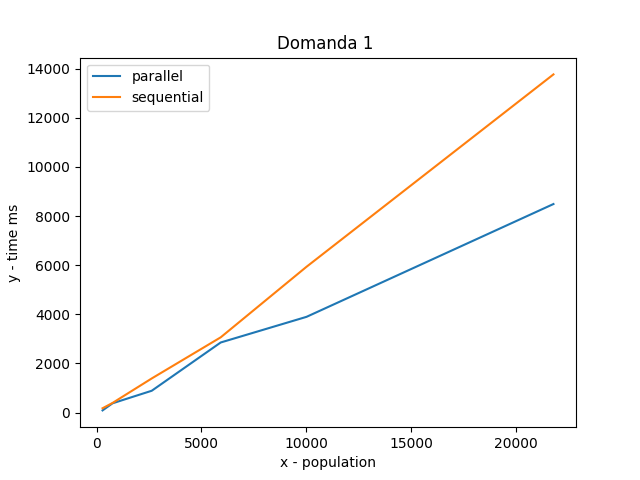
\includegraphics[width=1\linewidth, valign=t]{figures/domanda1}
	\end{figure}
\end{center}
Nel grafico vengono messi a confronto i tempi ottenuti dall'algormitmo k-means, nella sua versione parallela e sequenziale, al variare della popolazione tenendo costanti i parametri: 50 cluster, 100 iterazioni e cutoff 20.\\
Si è scelto di usare tale cutoff in quanto la versione puramente parallela (cutoff = 0) sarebbe stata penalizzata da un'onere eccessivo di runtime.\\
Come si evince dal grafico la versione parallela ottiene tempi sempre migliori rispetto alla controparte sequenziale.


\begin{center}
	\begin{figure}[H]
		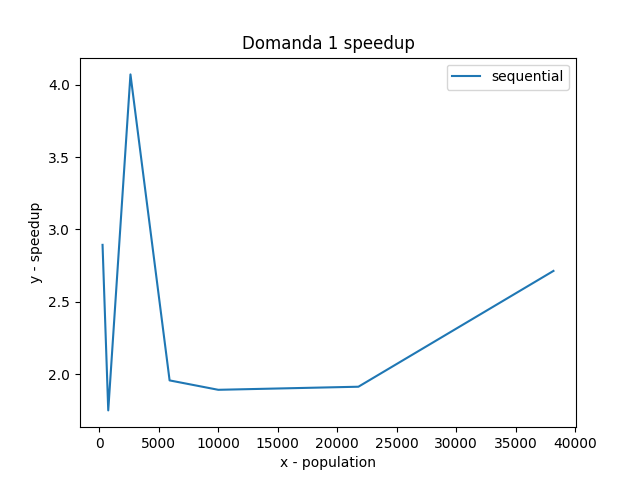
\includegraphics[width=1\linewidth, valign=t]{figures/domanda1speedup}
	\end{figure}
\end{center}
Il grafico mostra lo speedup calcolato come il rapporto tra i tempi dell'algoritmo k-means sequenziale e parallelo, al variare della popolazione. \\
Dai dati a disposizione sembra evincersi una tendenza positiva in quanto lo $speedup > 1$, inoltre si vede che all'aumentare della popolazione aumenta esso stesso.


\section*{Domanda 2}
\begin{center}
	\begin{figure}[H]
		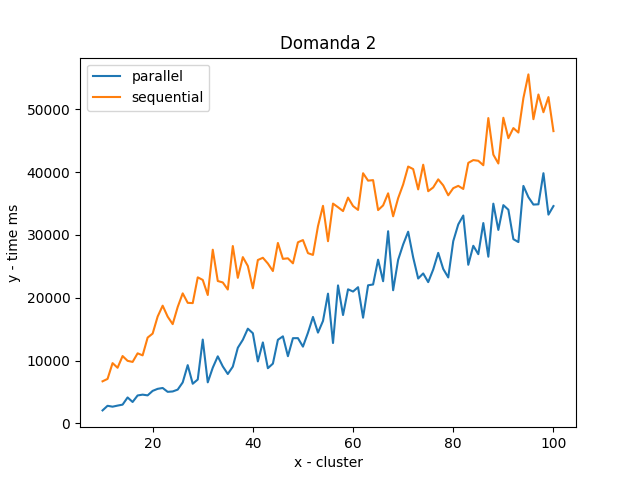
\includegraphics[width=1\linewidth, valign=t]{figures/domanda2}
	\end{figure}
\end{center}
Nel grafico vengono mostrati i tempi di esecuzione dell'algoritmo k-means parallelo e sequenziale, al variare del numero di cluster, calcolato sul dataset complessivo di 38183 punti, con 100 iterazioni e cutoff 20, si può vedere come l'algoritmo parallelo abbia tempi sempre migliori rispetto la controparte sequenziale.
	

\begin{center}
	\begin{figure}[H]
		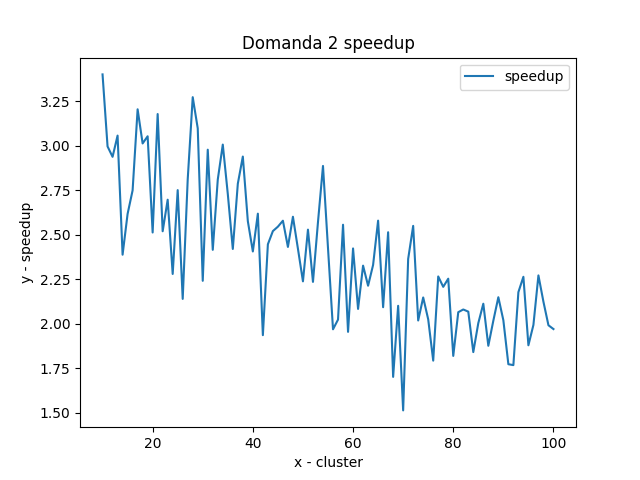
\includegraphics[width=1\linewidth, valign=t]{figures/domanda2speedup}
	\end{figure}
\end{center}
Il grafico mostra l'andamento dello speedup calcolato attraverso il rapporto tra i tempi dell'algoritmo k-means sequenziale e parallelo, al variare del numero di cluster. \\
Si evince come lo speedup abbia un andamento descrescente, all'aumentare del numero dei cluster, questo perché se aumenta il numero di cluster aumentano le ricerche in parallelo su tutti i punti per calcolare il nuovo centroide, cosa che invece non avviene nella versione sequenziale, in quanto i punti sono già divisi rispetto i cluster.



\section*{Domanda 3}
\begin{center}
	\begin{figure}[H]
		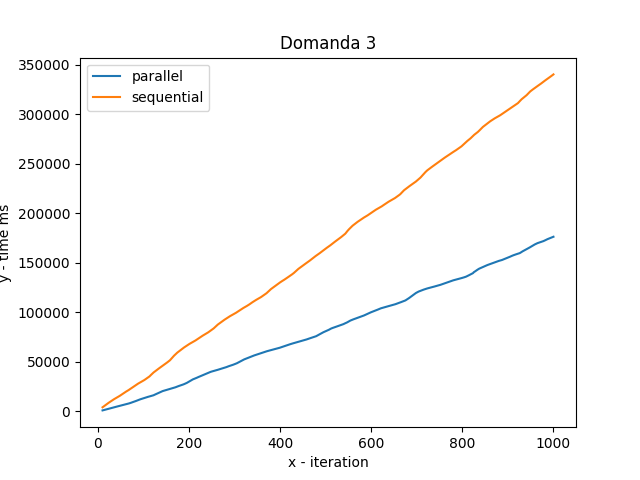
\includegraphics[width=1\linewidth, valign=t]{figures/domanda3}
	\end{figure}
\end{center}
Nel grafico vengono mostrati i tempi di esecuzione dell'algoritmo k-means parallelo e sequenziale, al variare del numero di iterazioni, calcolato sul dataset complessivo di 38183 punti, 50 cluster e cutoff 20, si può vedere come l'algoritmo parallelo abbia tempi sempre migliori rispetto la controparte sequenziale.
	

\begin{center}
	\begin{figure}[H]
		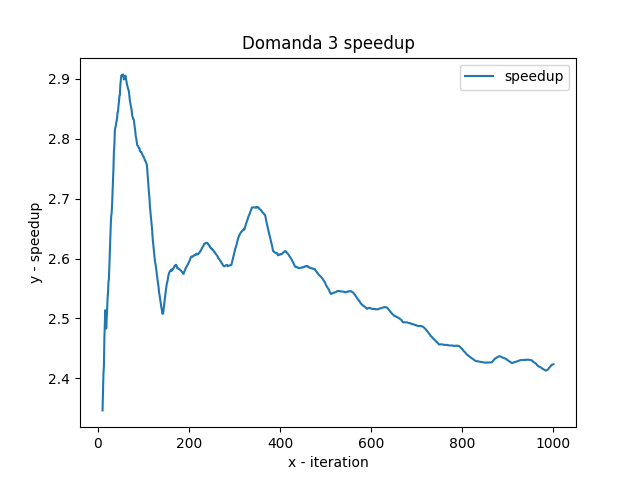
\includegraphics[width=1\linewidth, valign=t]{figures/domanda3speedup}
	\end{figure}
\end{center}
Il grafico mostra l'andamento dello speedup calcolato attraverso il rapporto tra i tempi dell'algoritmo k-means sequenziale e parallelo, al variare del numero di iterazioni. Si evince come lo speedup abbia un andamento descrescente, all'aumentare del numero dei iterazioni, attestandosi nella parte finale (iterazioni $\;\approx 1000$) a circa 2.


\section*{Domanda 4}
\begin{center}
	\begin{figure}[H]
		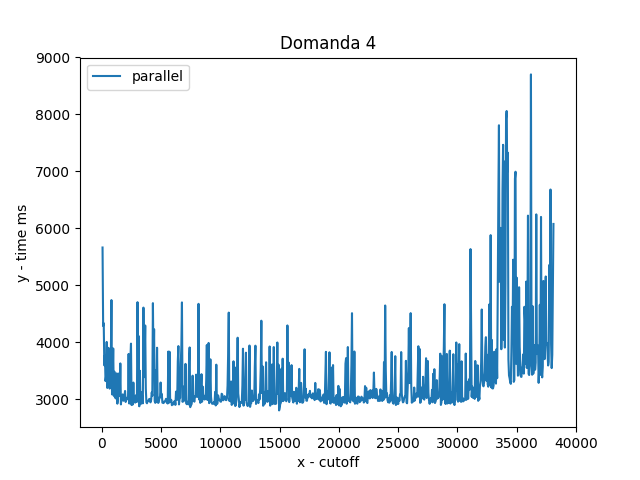
\includegraphics[width=1\linewidth, valign=t]{figures/domanda4}
	\end{figure}
					
\end{center}

\noindent Nel grafico vengono mostrati i tempi di esecuzione dell'algoritmo k-means parallelo, al variare del cutoff, calcolato sul dataset complessivo di 38183 punti, 50 cluster, 100 iterazioni e con un passo tra un cutoff e il successivo pari a 50.\\ 
							
\newpage	
\begin{wrapfigure}[12]{l}{6cm}
	\vspace*{-0.5cm}
	\centering
	\begin{tabular}{lcc}
		\toprule
		$min_{cutoff}$ & $max_{cutoff}$ & Thread  \\
		\midrule
		38183          & 38183          & 1       \\
		19091          & 38182          & 2       \\
		9545           & 190910         & 4       \\
		4772           & 9544           & 8       \\
		2386           & 4771           & 16      \\
		$\dots$        & $\dots$        & $\dots$ \\
		0              & 0              & 38183   \\			
		\bottomrule
	\end{tabular}
\end{wrapfigure}

\noindent Come sottolineato dall'andamento a gradoni e facendo riferimento alla tabella riportata qui di fianco, si può vedere come per intervalli di cutoff via via sempre più piccoli rispetto al massimo rappresentante di cutoff disponibile, il tempo di esecuzione tende a rudirsi.\\ Trovandosi ad avere cutoff molto bassi si può dire di essere in prossimità di un parallelismo puro (cutoff$\;\approx 0$) mentre per cutoff molto alti ci si trova in prossimità della versione della versione sequenziale dell'algoritmo (cutoff$\;\approx 38183$).\\ Possiamo notare come per cutoff appartenenti allo stesso intervallo si abbiano tempi di esecuzione simili.\\
				
\noindent L'algoritmo parallelo da il meglio di sè utilizzando un cutoff compreso nell'intervallo $[500,5000]$, ne troppo basso (parallelismo perfetto), ne troppo alto (praticamente sequenziale), favorendo quindi una versione ibrida.

\section*{Domanda 5}
Il computer su cui sono stati eseguiti i test dispone del seguente processore: \textit{Intel(R) Core(TM) i7-2820QM CPU\\ Clockspeed: 2.3 GHz, Turbo Speed: 3.4 GHz\\ Number of Cores: 4 (2 logical cores per physical)}.

\section*{Domanda 6}
Per sviluppare le domande della relazione abbiamo creato un file \textit{istance.csv} al cui interno abbiamo inserito per ogni riga un'istanza da eseguire nel seguente formato: $$\textbf{dom,pop,k,it,cutoff}$$
Per lanciare l'esecuzione si deve eseguire il seguente comando \textit{go run ./main.go ./kmeans.go ./parser.go}.
I risultati verranno inseriti nello stesso ordine di quello dell'input all'interno del file \textit{result.csv} nel seguente formato: $$\textbf{dom\;pop\;k\;it\;cutoff\;tempo\_par\;tempo\_seq}$$
\end{document}


